\section{Square lattice}
\label{sec:square}

Similarly to what happens for the \acs{1D} case, both mean field and \ac{QMC} results for the square lattice suggest that at half filling, \ac{AF} order persists in the ground state for any value of the on-site interaction \cite{claveau_mean-field_2014, gouveia_magnetic_2015, white_numerical_1989, hirsch_two-dimensional_1985}

\begin{figure}[H]
\label{fig:mfHubbardPhaseDiagram}
\hspace{-0.18cm}
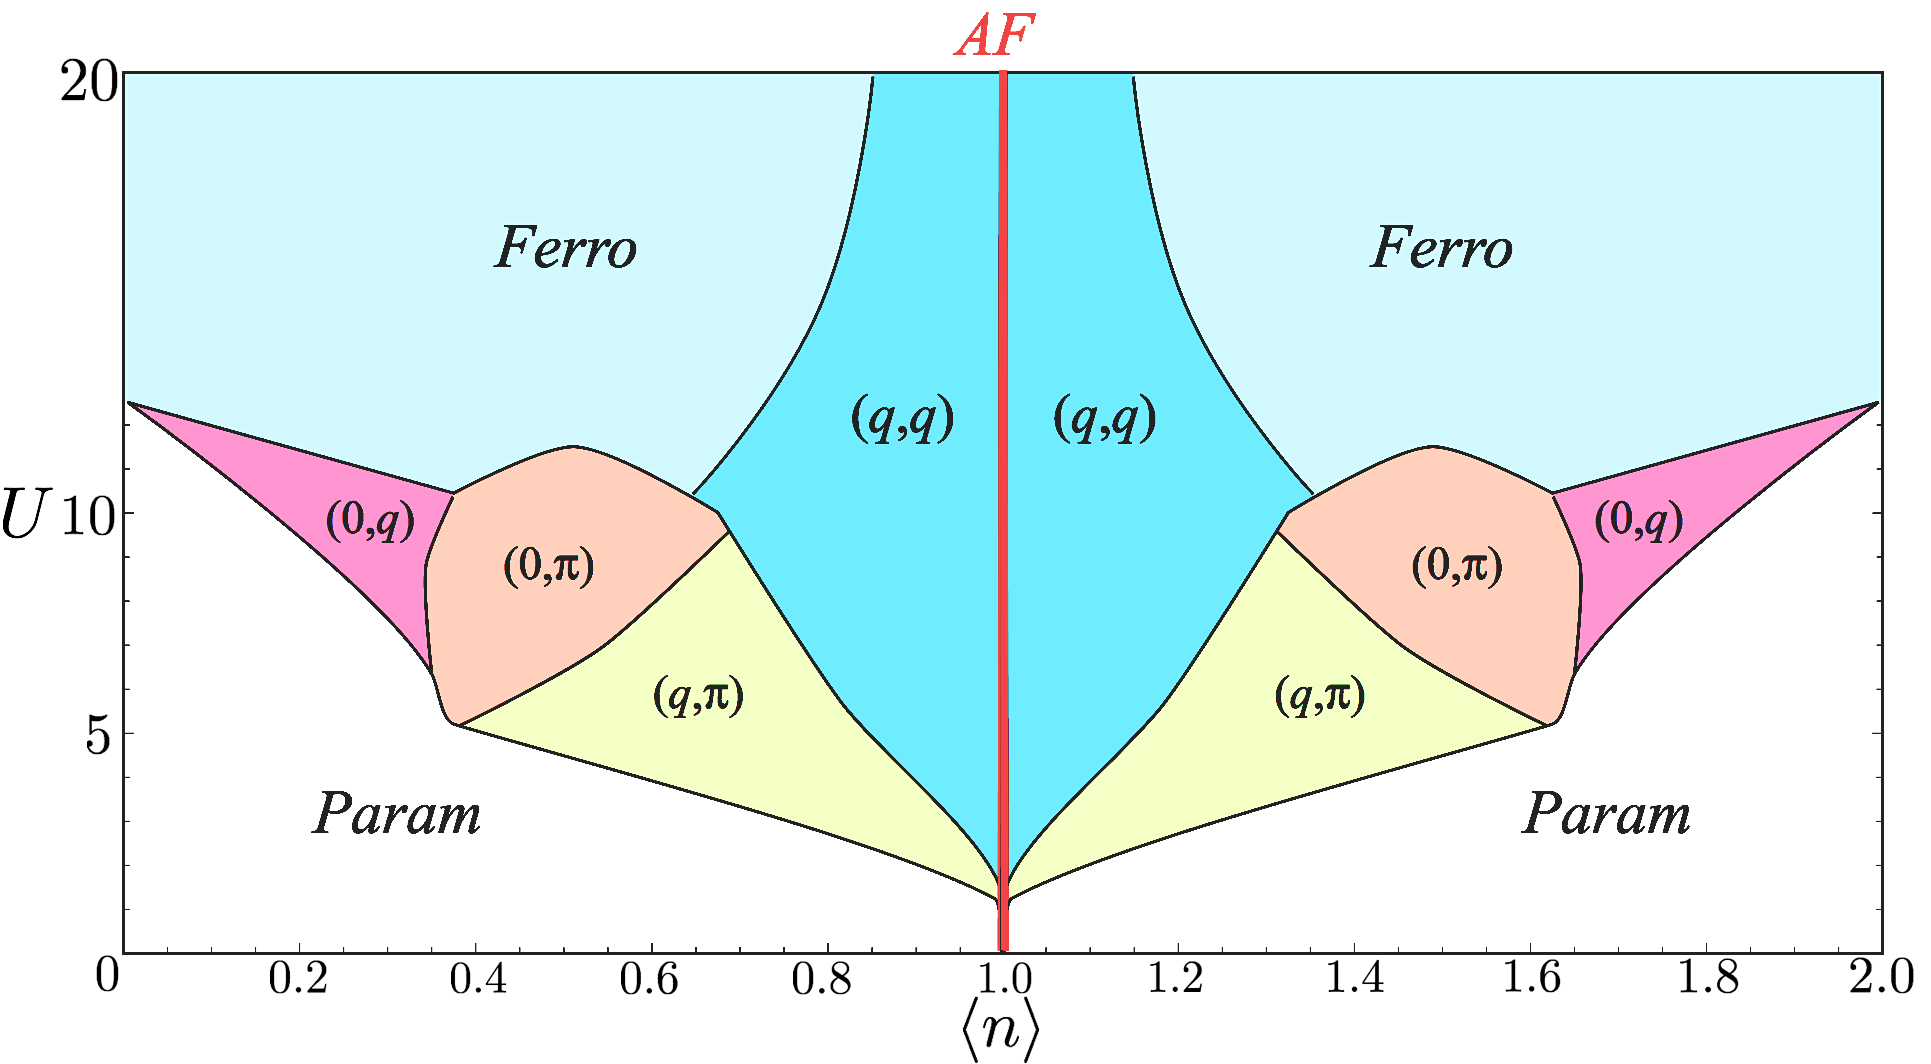
\includegraphics[scale=0.245]{Applications/mf-phase-diagram-hubbard}
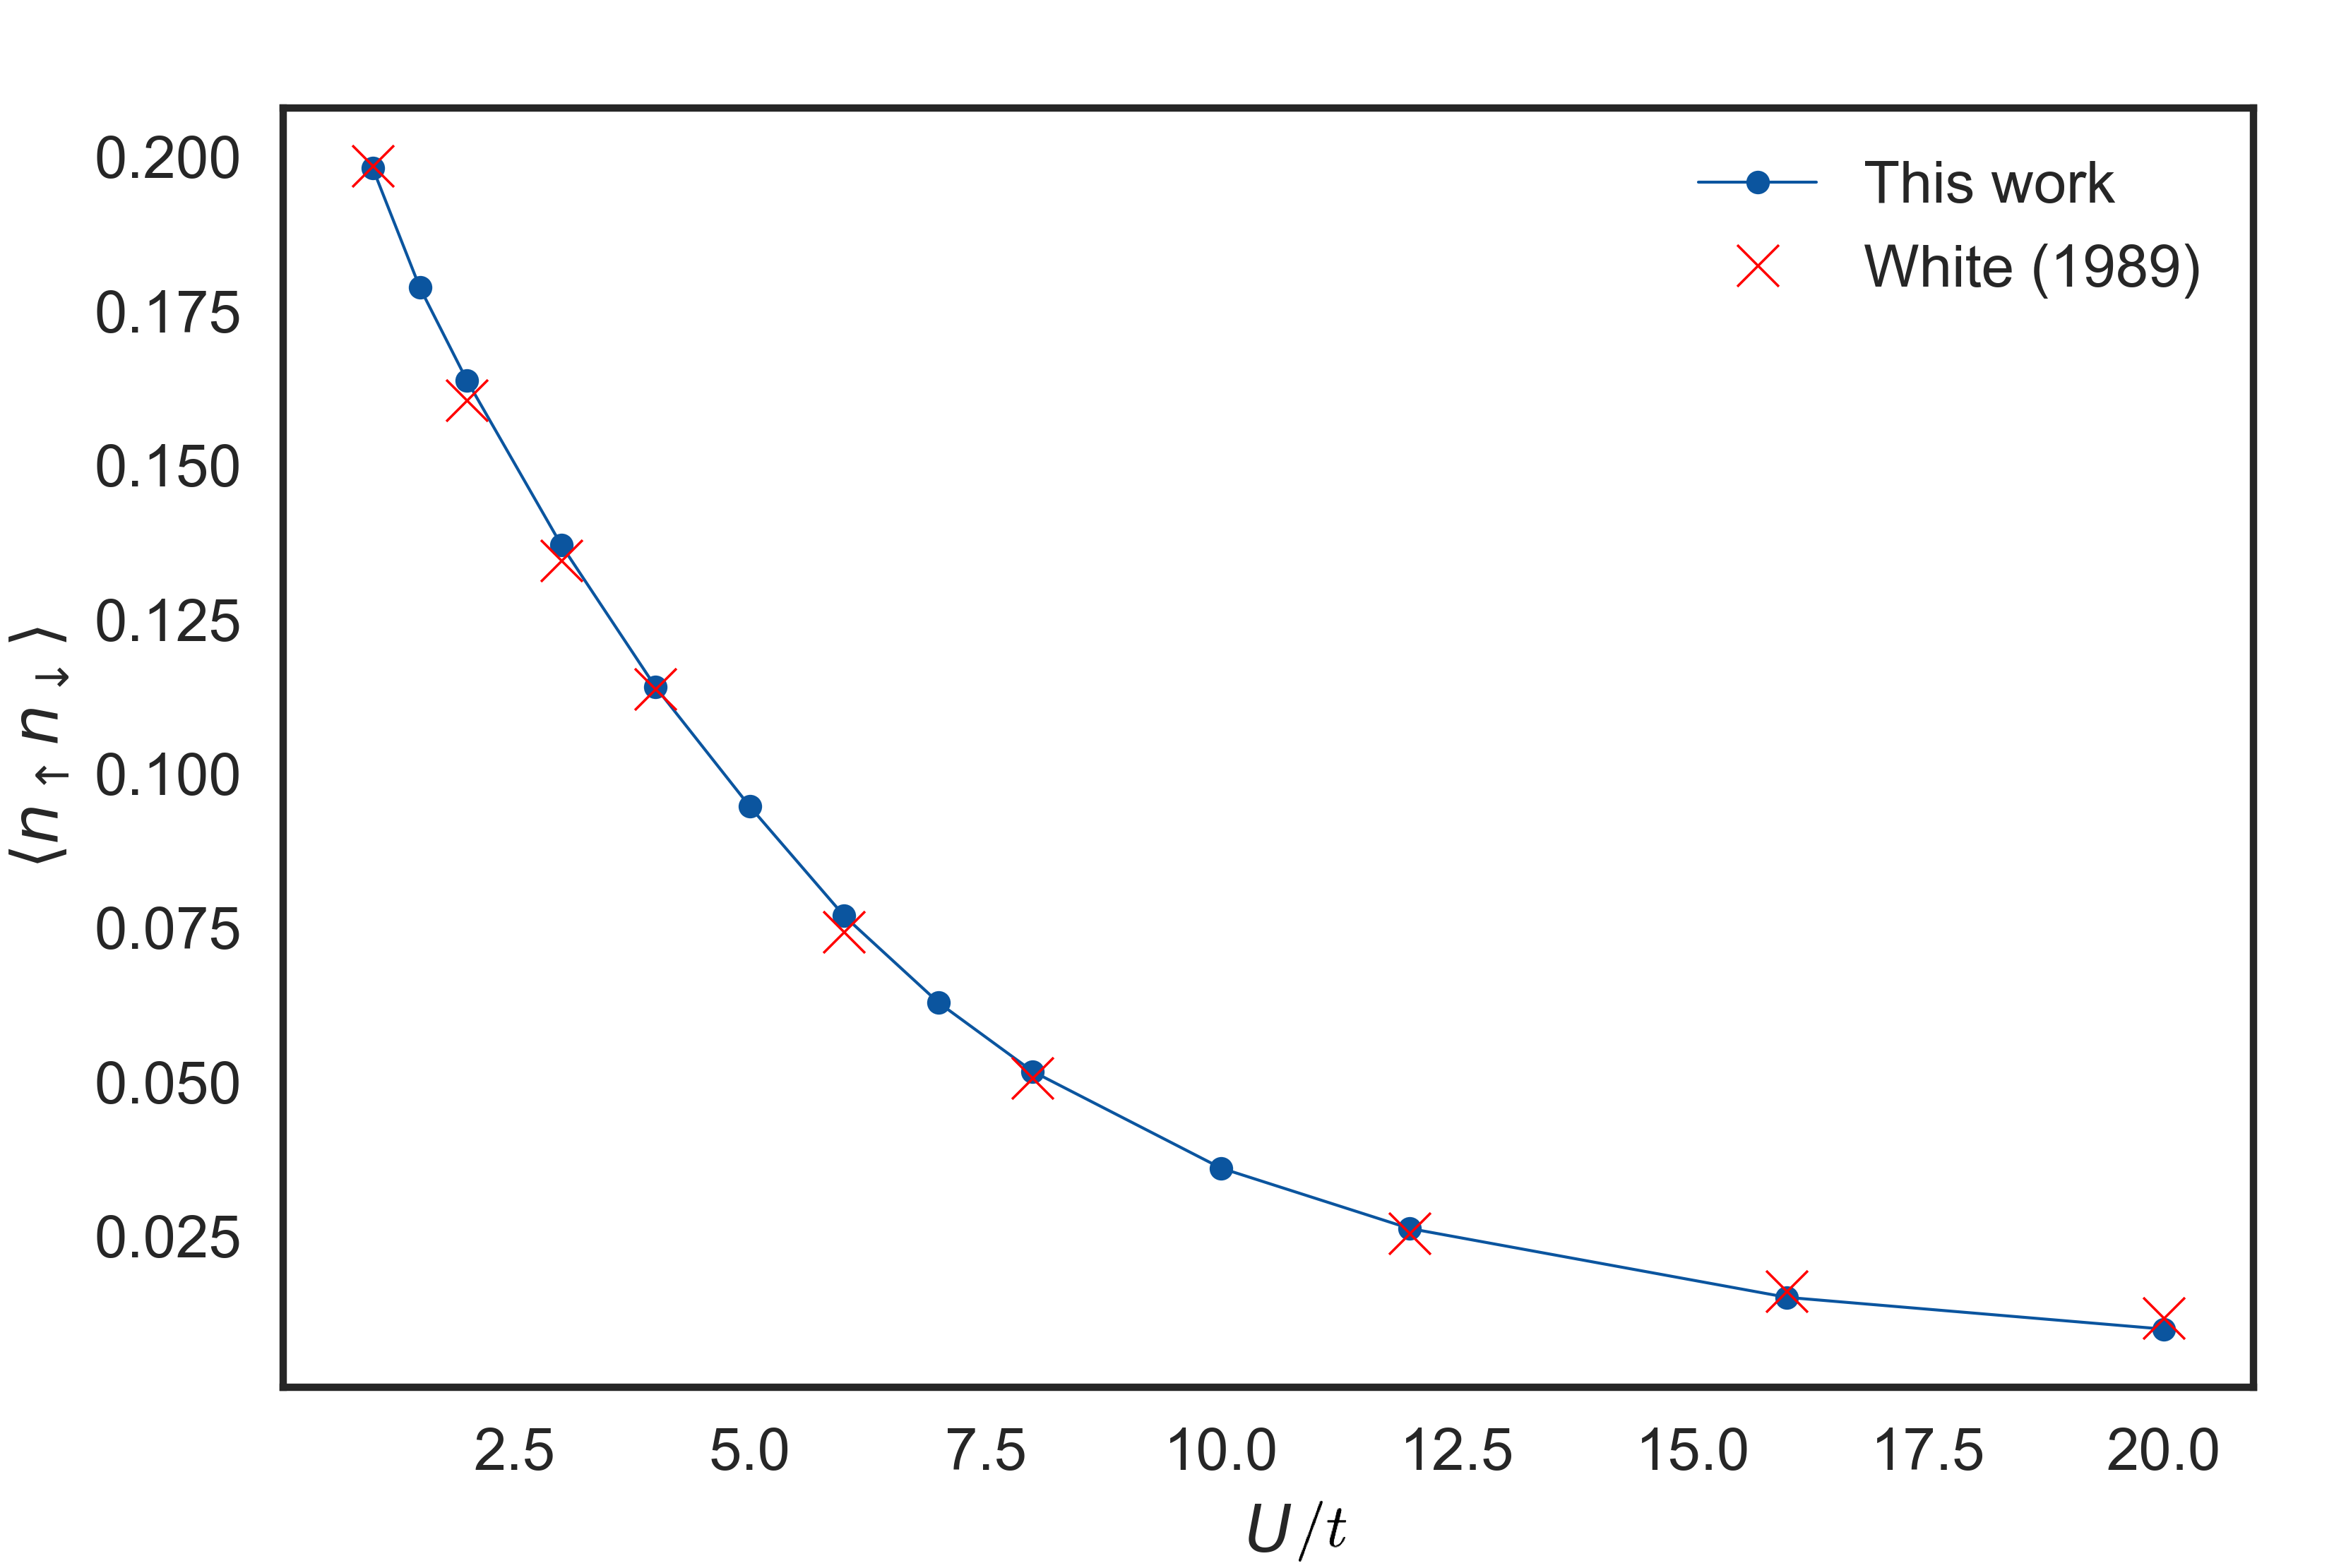
\includegraphics[scale=0.493]{Applications/square/nUpnDwSquare}
\caption[Mean field phase diagram of the Hubbard model. \ac{QMC} data showing the decrease of the double occupancy with increasing $U$.]{Left: MF phase diagram of the Hubbard model \cite{gouveia_magnetic_2015}.
Right: \ac{QMC} data showing the decrease of the double occupancy with increasing $U$, reproducing the results of \cite{white_numerical_1989}.}
\end{figure}
Our results for a half-filled $4 \times 4$ lattice at $\beta = 16 t$ clearly show antiferromagnetic spin-spin correlations - Fig.(\ref{fig:corrSq},left), which results in a peak of the magnetic structure factor $S (\bm q)$ at $\bm q = (\pi, \pi)$ - Fig.(\ref{fig:corrSq},right).
\begin{figure}[H]
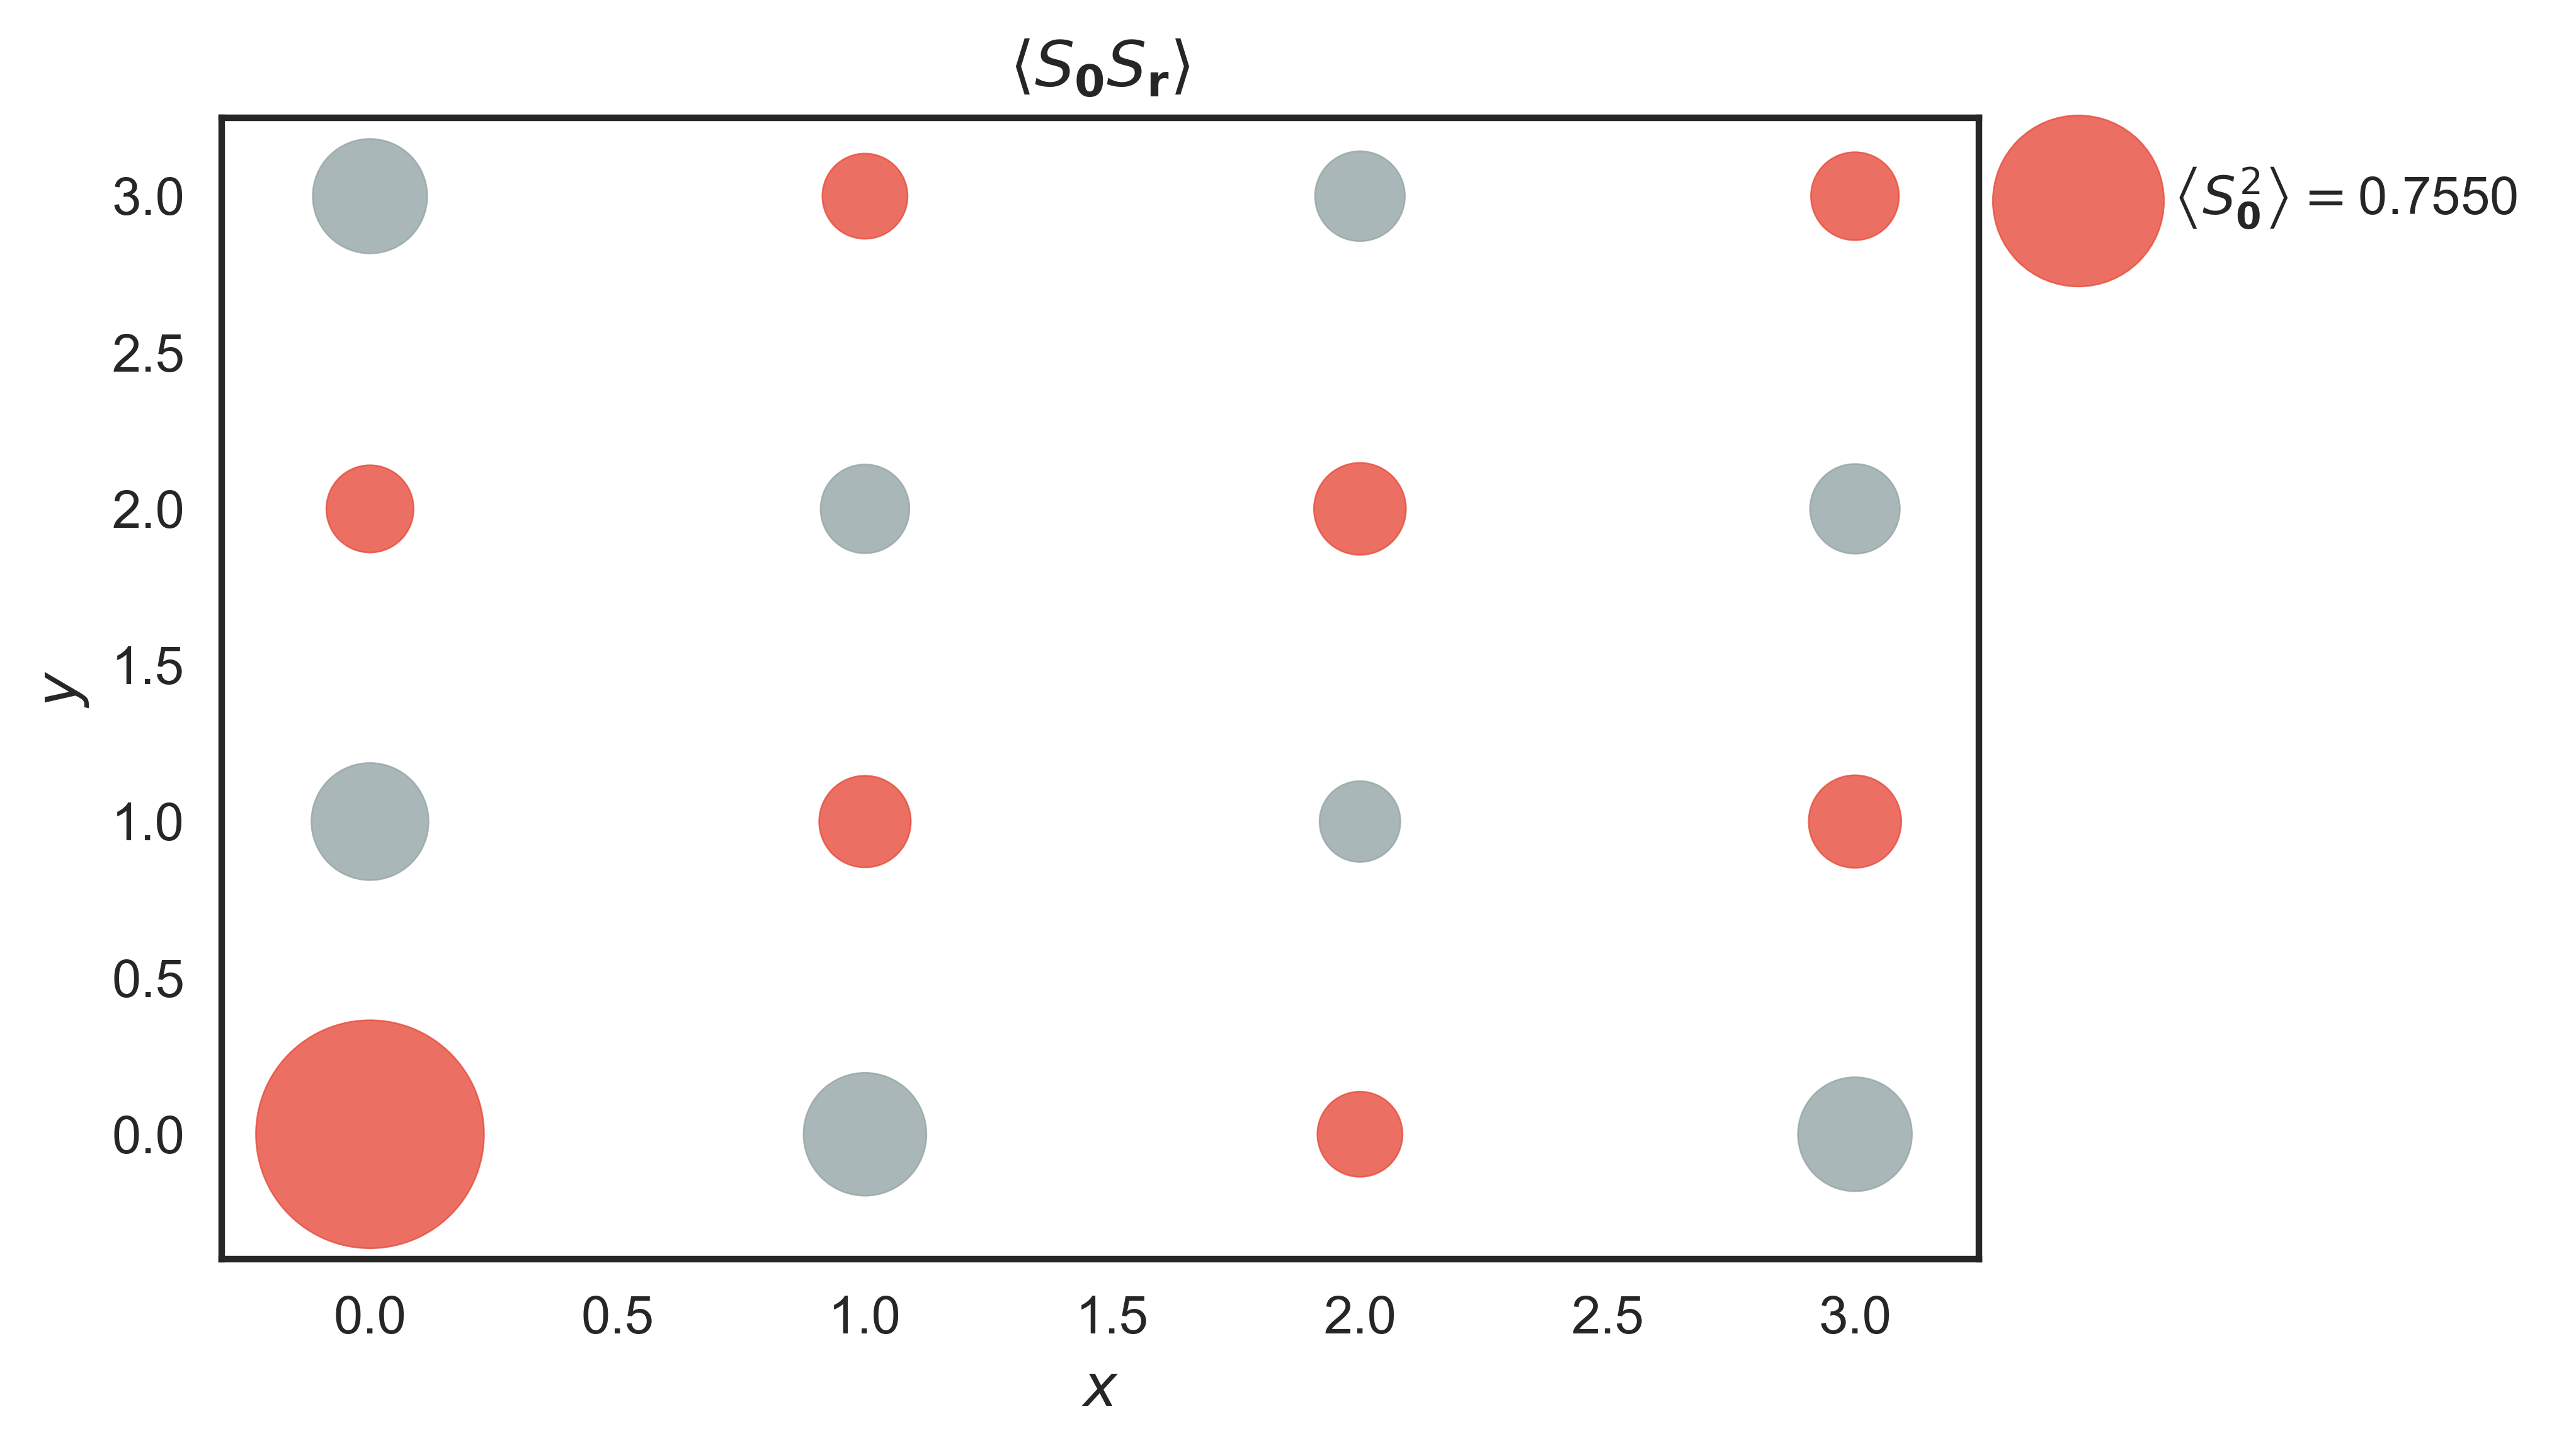
\includegraphics[scale=0.55]{Applications/square/CorrelationsDots}
\hspace{0.5cm}
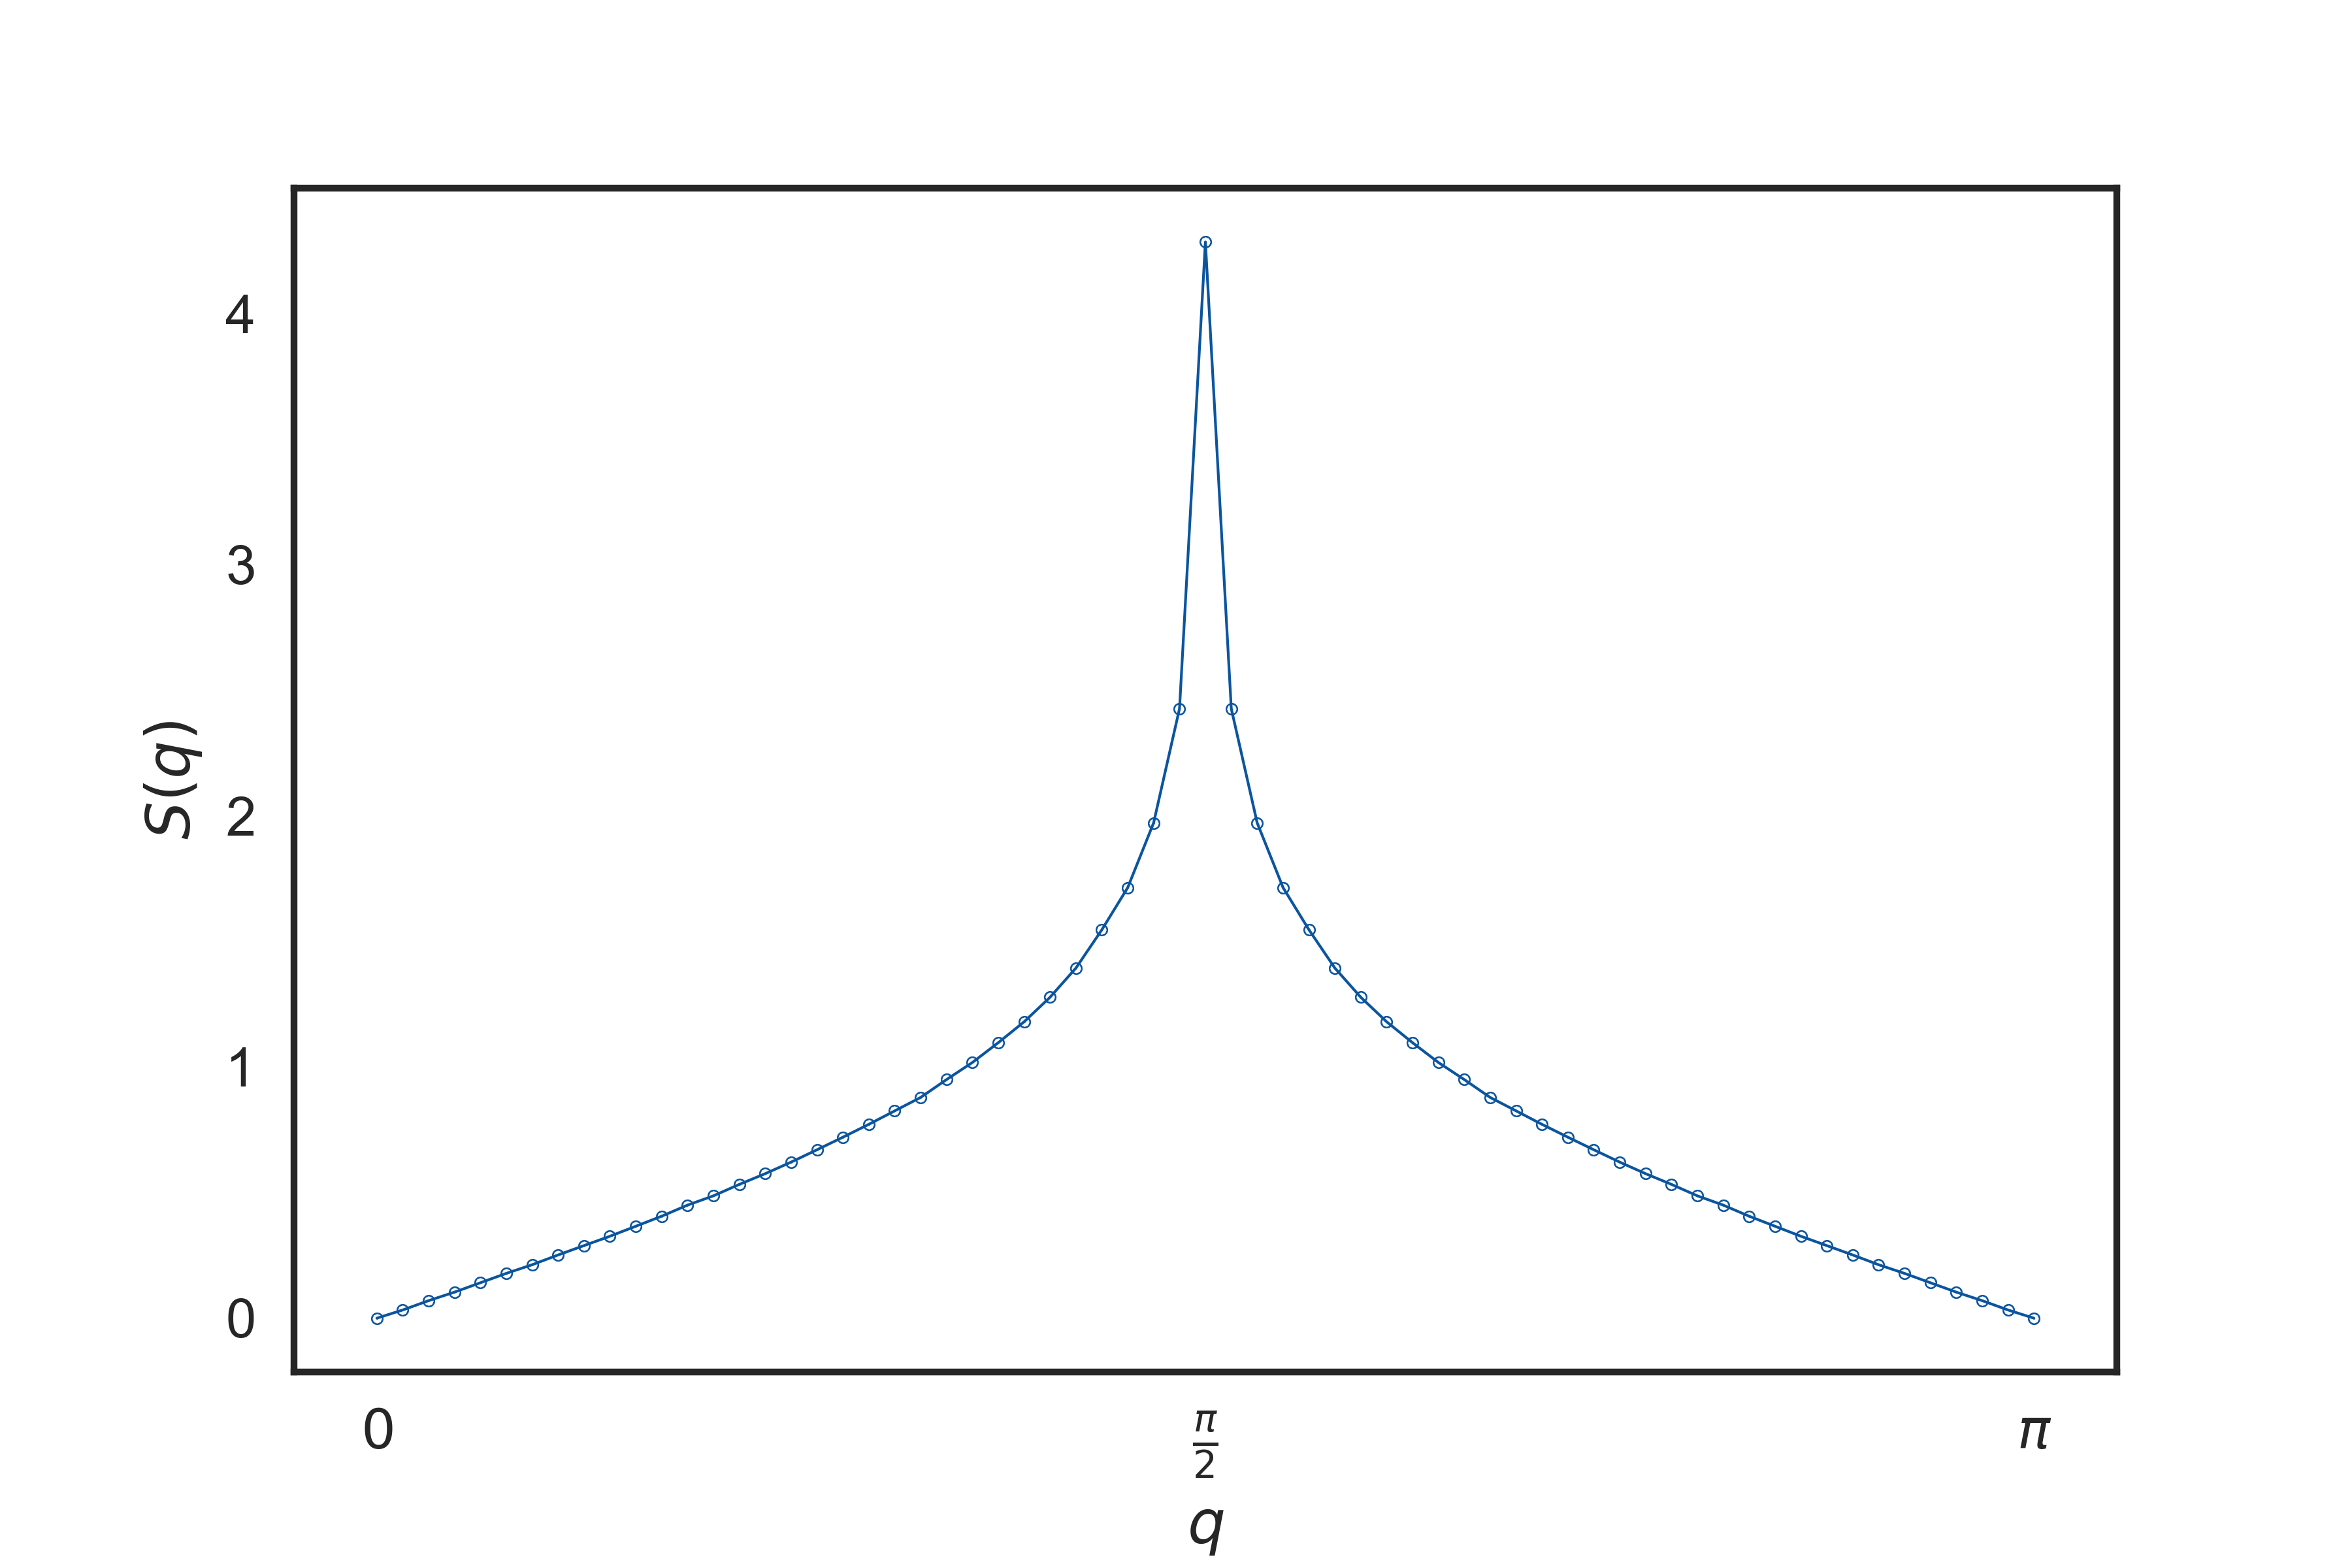
\includegraphics[scale=0.65]{Applications/square/S(q)}
\caption[Spin-spin correlations on the square lattice.
Magnetic structure factors showing a peak at $\bm q = \bm \pi$.]{Spin-spin correlations with respect to the point on the lower left corner of the lattice (which we label as $\bm 0$).
3D Plot of the magnetic structure factor $S ( \bm q)$ displaying the $\bm q = \bm \pi$ peak \label{fig:corrSq}.}
\end{figure}
The susceptibility $\chi ( \bm q) $ is also strongly peaked at $\bm q = \bm \pi$, again revealing long range \ac{AF} order.
\begin{figure}[H]
\hspace{1cm}
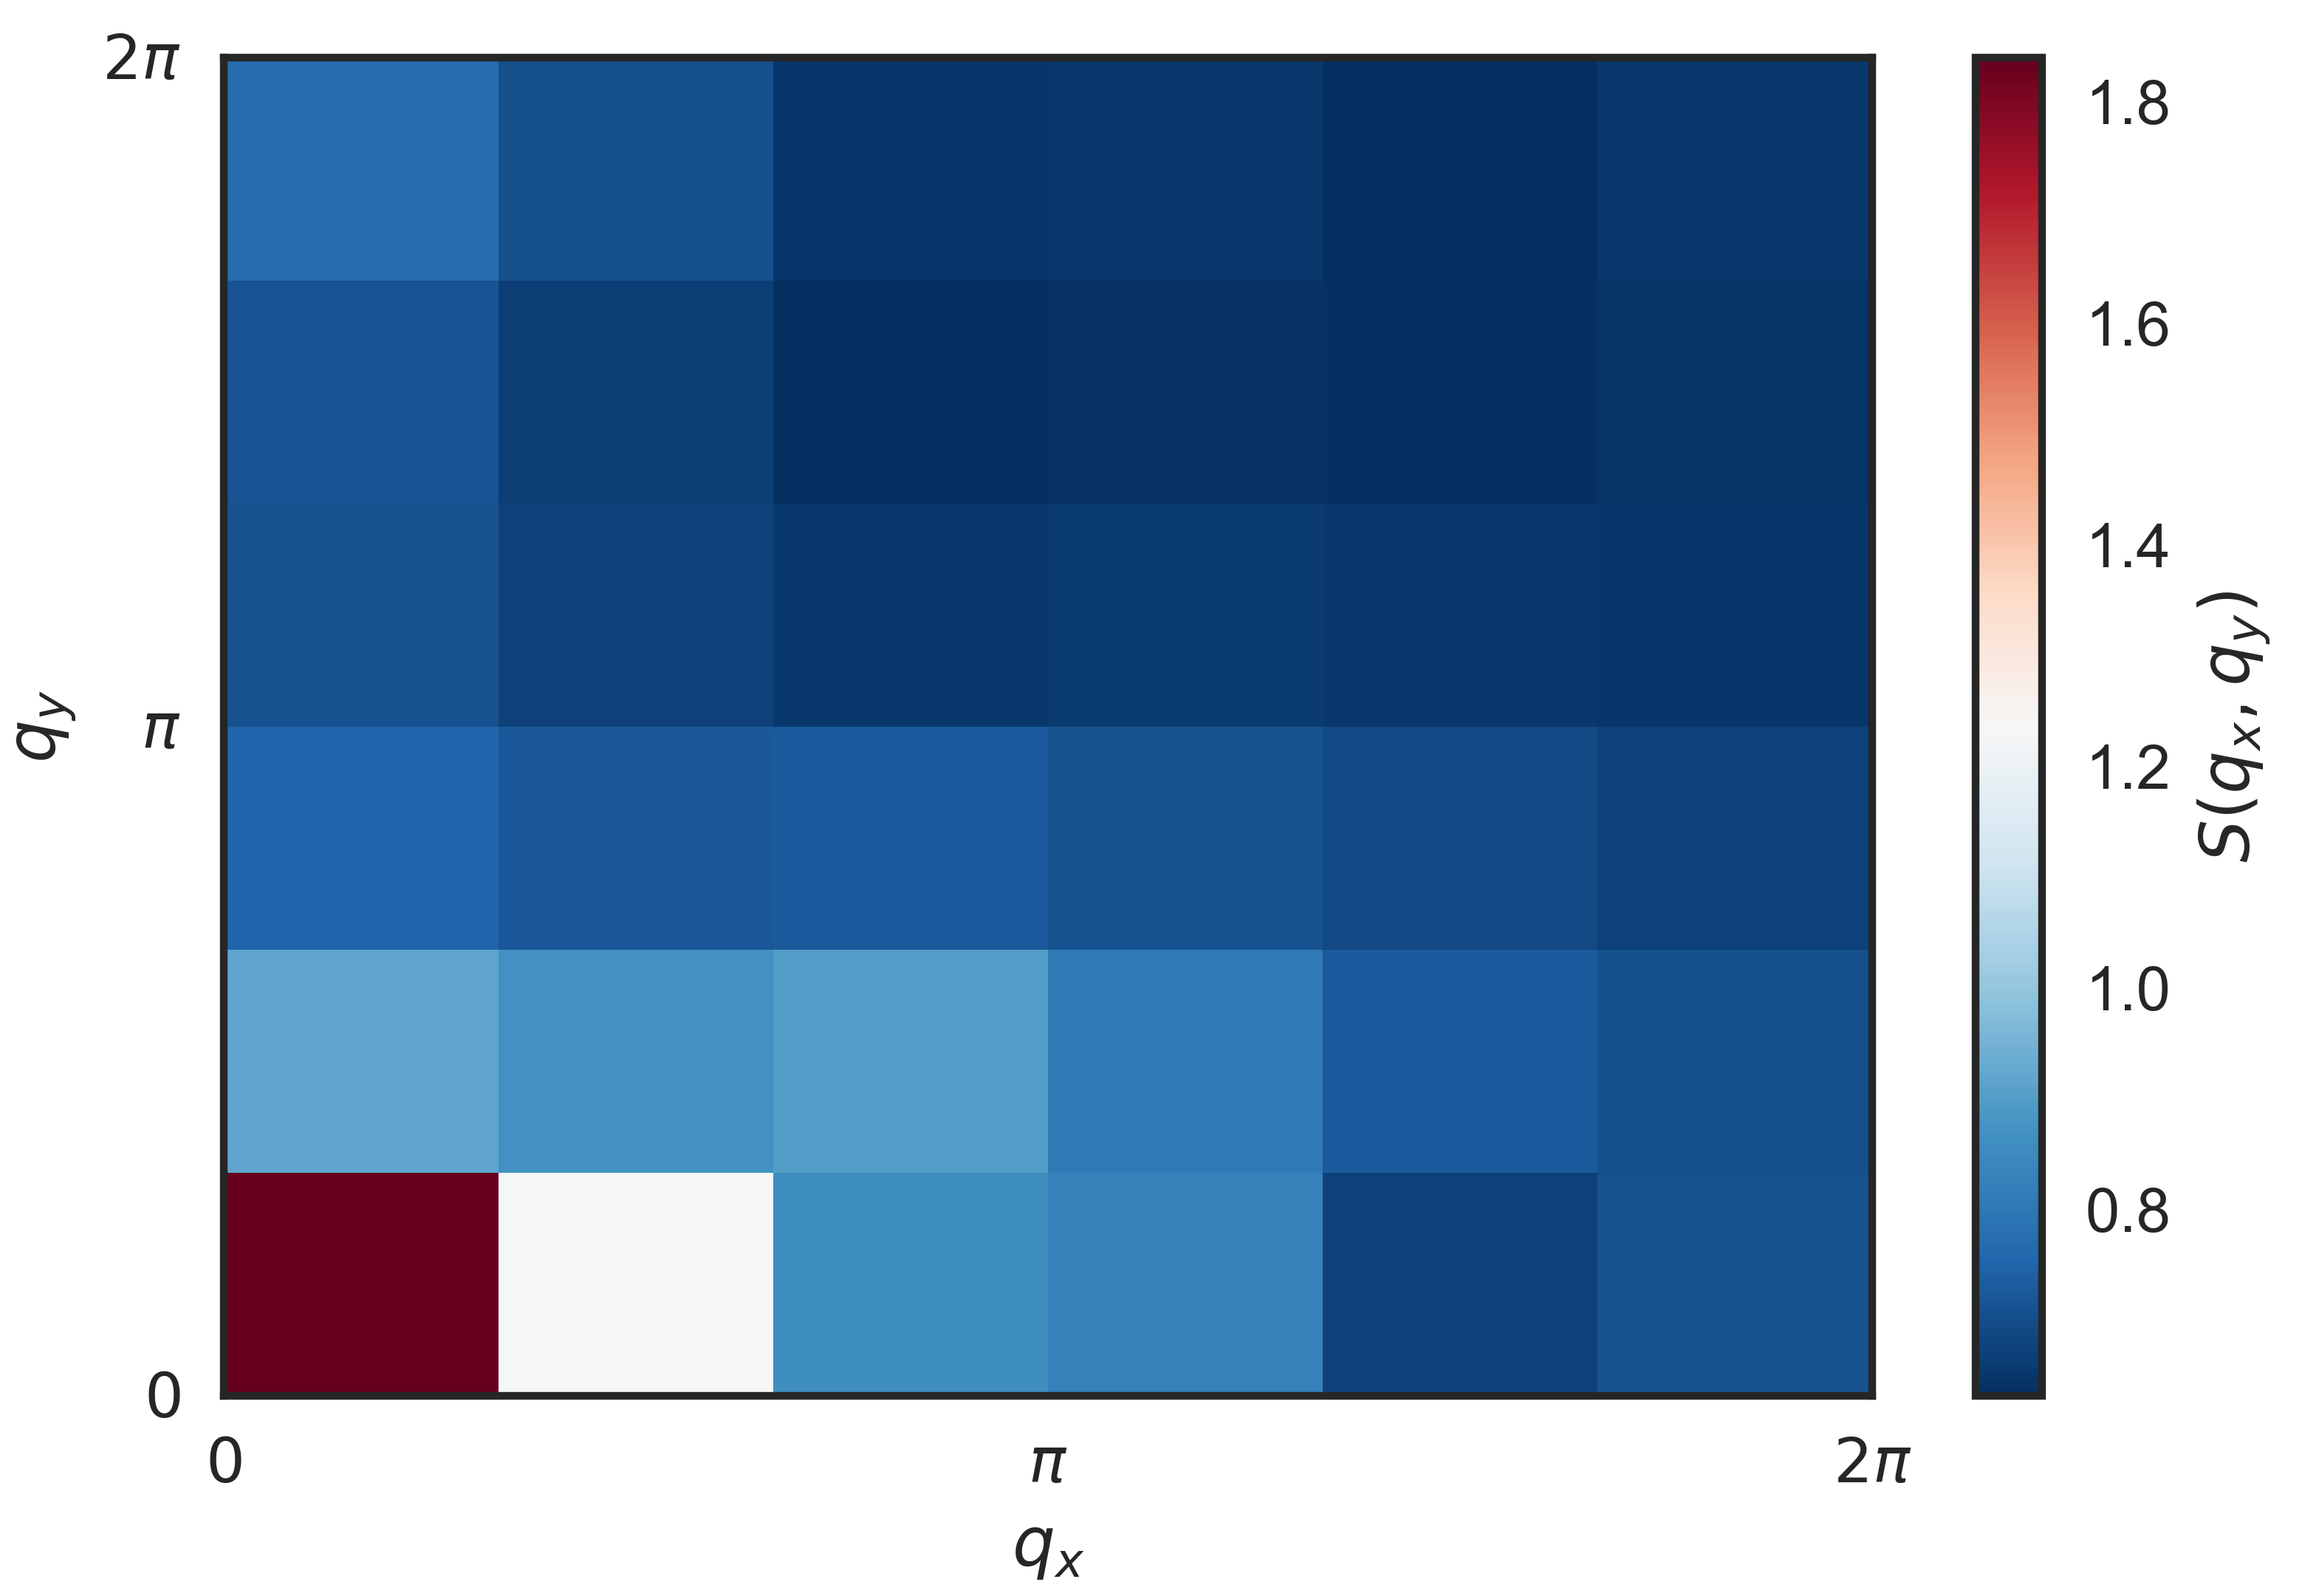
\includegraphics[scale=0.5]{Applications/square/S(q)pcolor.png}
\hspace{0.4cm}
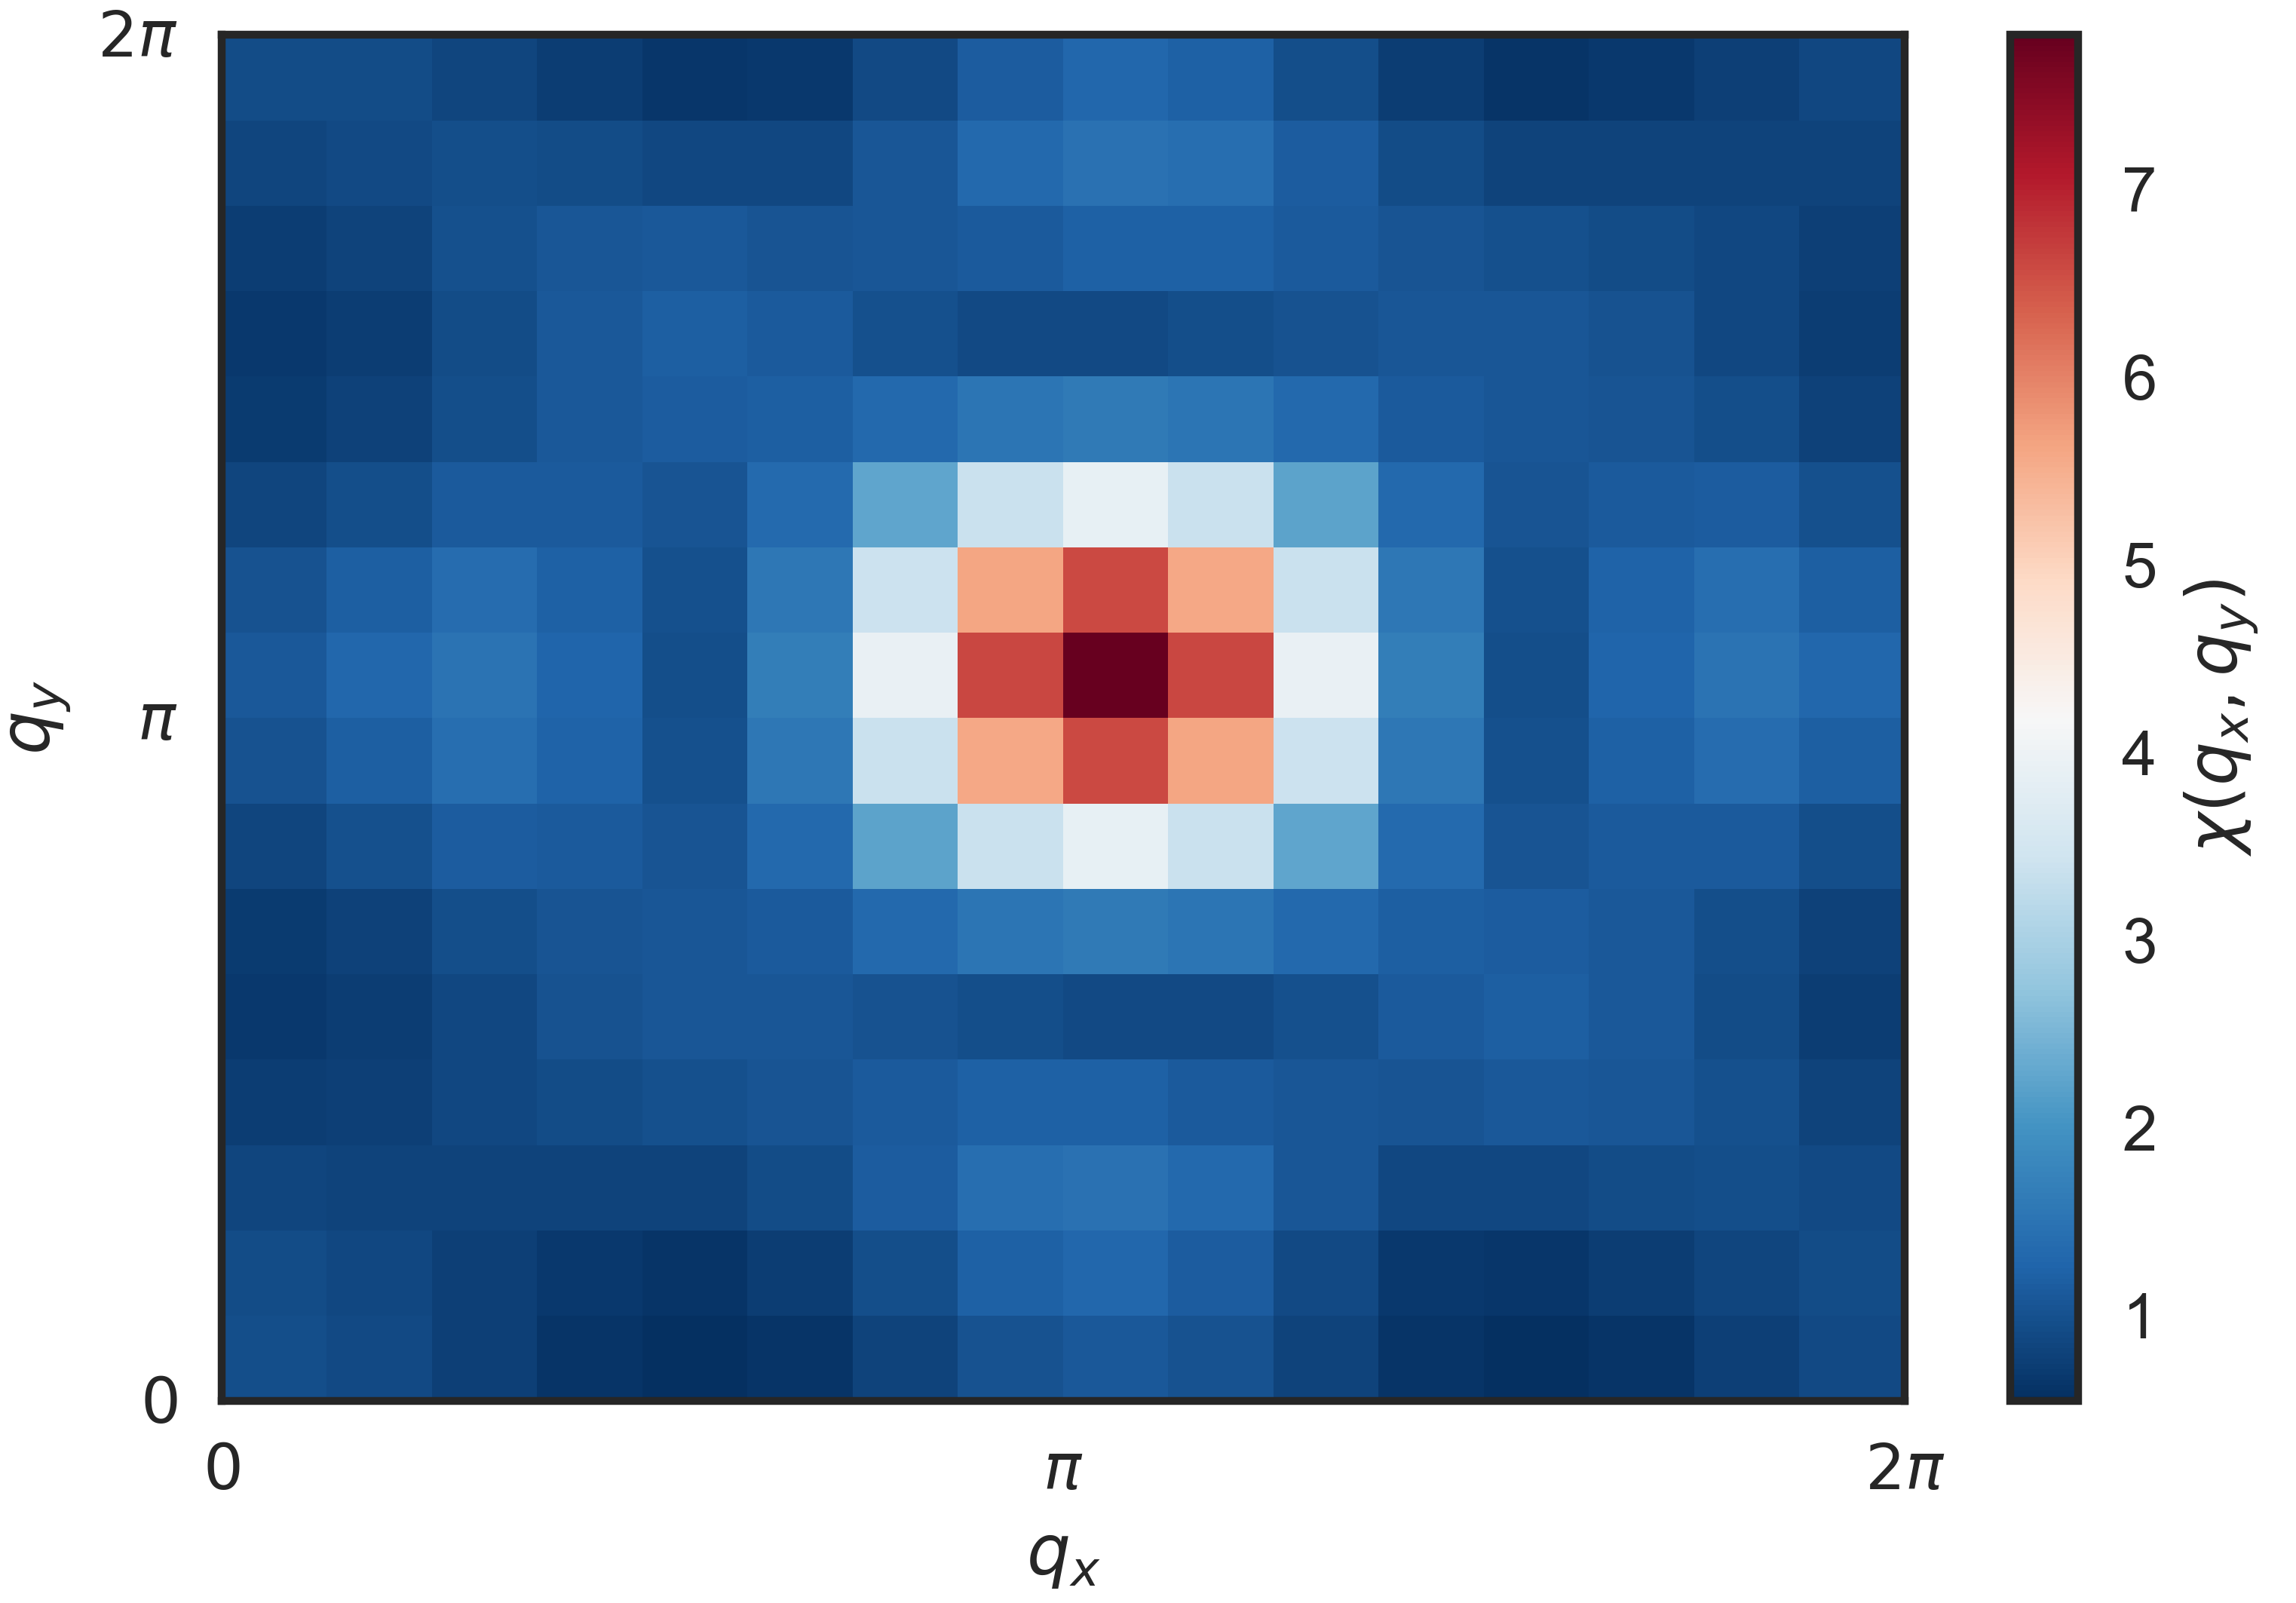
\includegraphics[scale=0.5]{Applications/square/chi(q)pcolor.png}
\caption[Color map of the structure factor $S ( \bm q)$, and susceptibility $\chi ( \bm q)$, both showing peaks at $\bm q = \bm\pi$.]{Color map of the structure factor $S ( \bm q)$, and susceptibility $\chi ( \bm q)$, both showing peaks at $\bm q = \bm\pi$.\label{fig:Schi3d}}
\end{figure}
\vspace{-0.5cm}
We finish this section by characterizing \ac{AF} order for varying system size and temperature, reproducing one of the main results of the seminal \ac{QMC} study of White, Scalapino and Sugar \cite{white_numerical_1989}.
In this paper, the authors report that by $\beta = 20 t$, our finite temperature algorithm is already measuring ground state properties.
In fact, for $\beta = 20 t$ the peaks $S ( \bm \pi )$ coincide with those obtained using the projective variant of auxiliary field \ac{QMC} mentioned in chapter \ref{cap:int}.
Extrapolating to the infinite system, we verify that long range order exists, i.e. the antiferromagnetic order parameter, or staggered magnetization is finite for $N \rightarrow \infty$.
Looking at Fig(\ref{fig:spipi}), it is clear that the zero temperature extrapolation of $\bm S (\pi)$ increases with lattice size.
In fact, as per \cite{hirsch_two-dimensional_1985}, for a sufficiently long lattice, at $T= 0$, we have that
\begin{equation}
S(\bm \pi) = N m_{\text{st}}^2 + S_c ( \bm \pi ) ,
\end{equation}
where $S_c ( \bm \pi )$ is the connected structure factor, obtained by replacing the average $\left\langle S^z_i S^z_j \right\rangle$ in the Fourier transform by $\left\langle S^z_i S^z_j \right\rangle - \left\langle S^z_i \right\rangle \left\langle S^z_j \right\rangle$, and $m_{\text{st}}$ is the \ac{AF} order parameter, or staggered magnetization:
\begin{equation}
m_{\text{st}} = \frac{1}{N} \sum_i (-1)^{R_i} \left\langle n_{i,\uparrow} - n_{i,\downarrow} \right\rangle
\end{equation}
Thus, to extrapolate the long range order, we fit $S ( \bm \pi ) / N$ by linear regression and obtain the estimate of the \ac{AF} order parameter as $m_{\text{st}}^2 = 0.09$.
As we increase $U$, this value becomes larger.
According to \cite{hirsch_two-dimensional_1985} (and references therein), on a finite lattice, the \ac{AF} long range order is $50 \%$ reduced from the classical Néel state due to quantum fluctuations.
Thus, at $U \rightarrow \infty$, we obtain the maximum value $m_{\text{st}}^2 = 0.25$.
Thus, the estimate we get for $m_{\text{st}}^2$  at $U=4$ amounts to $36\%$ of the maximum of $m_{\text{st}}^2$.
\vspace{-0.3cm}
\begin{figure}[H]
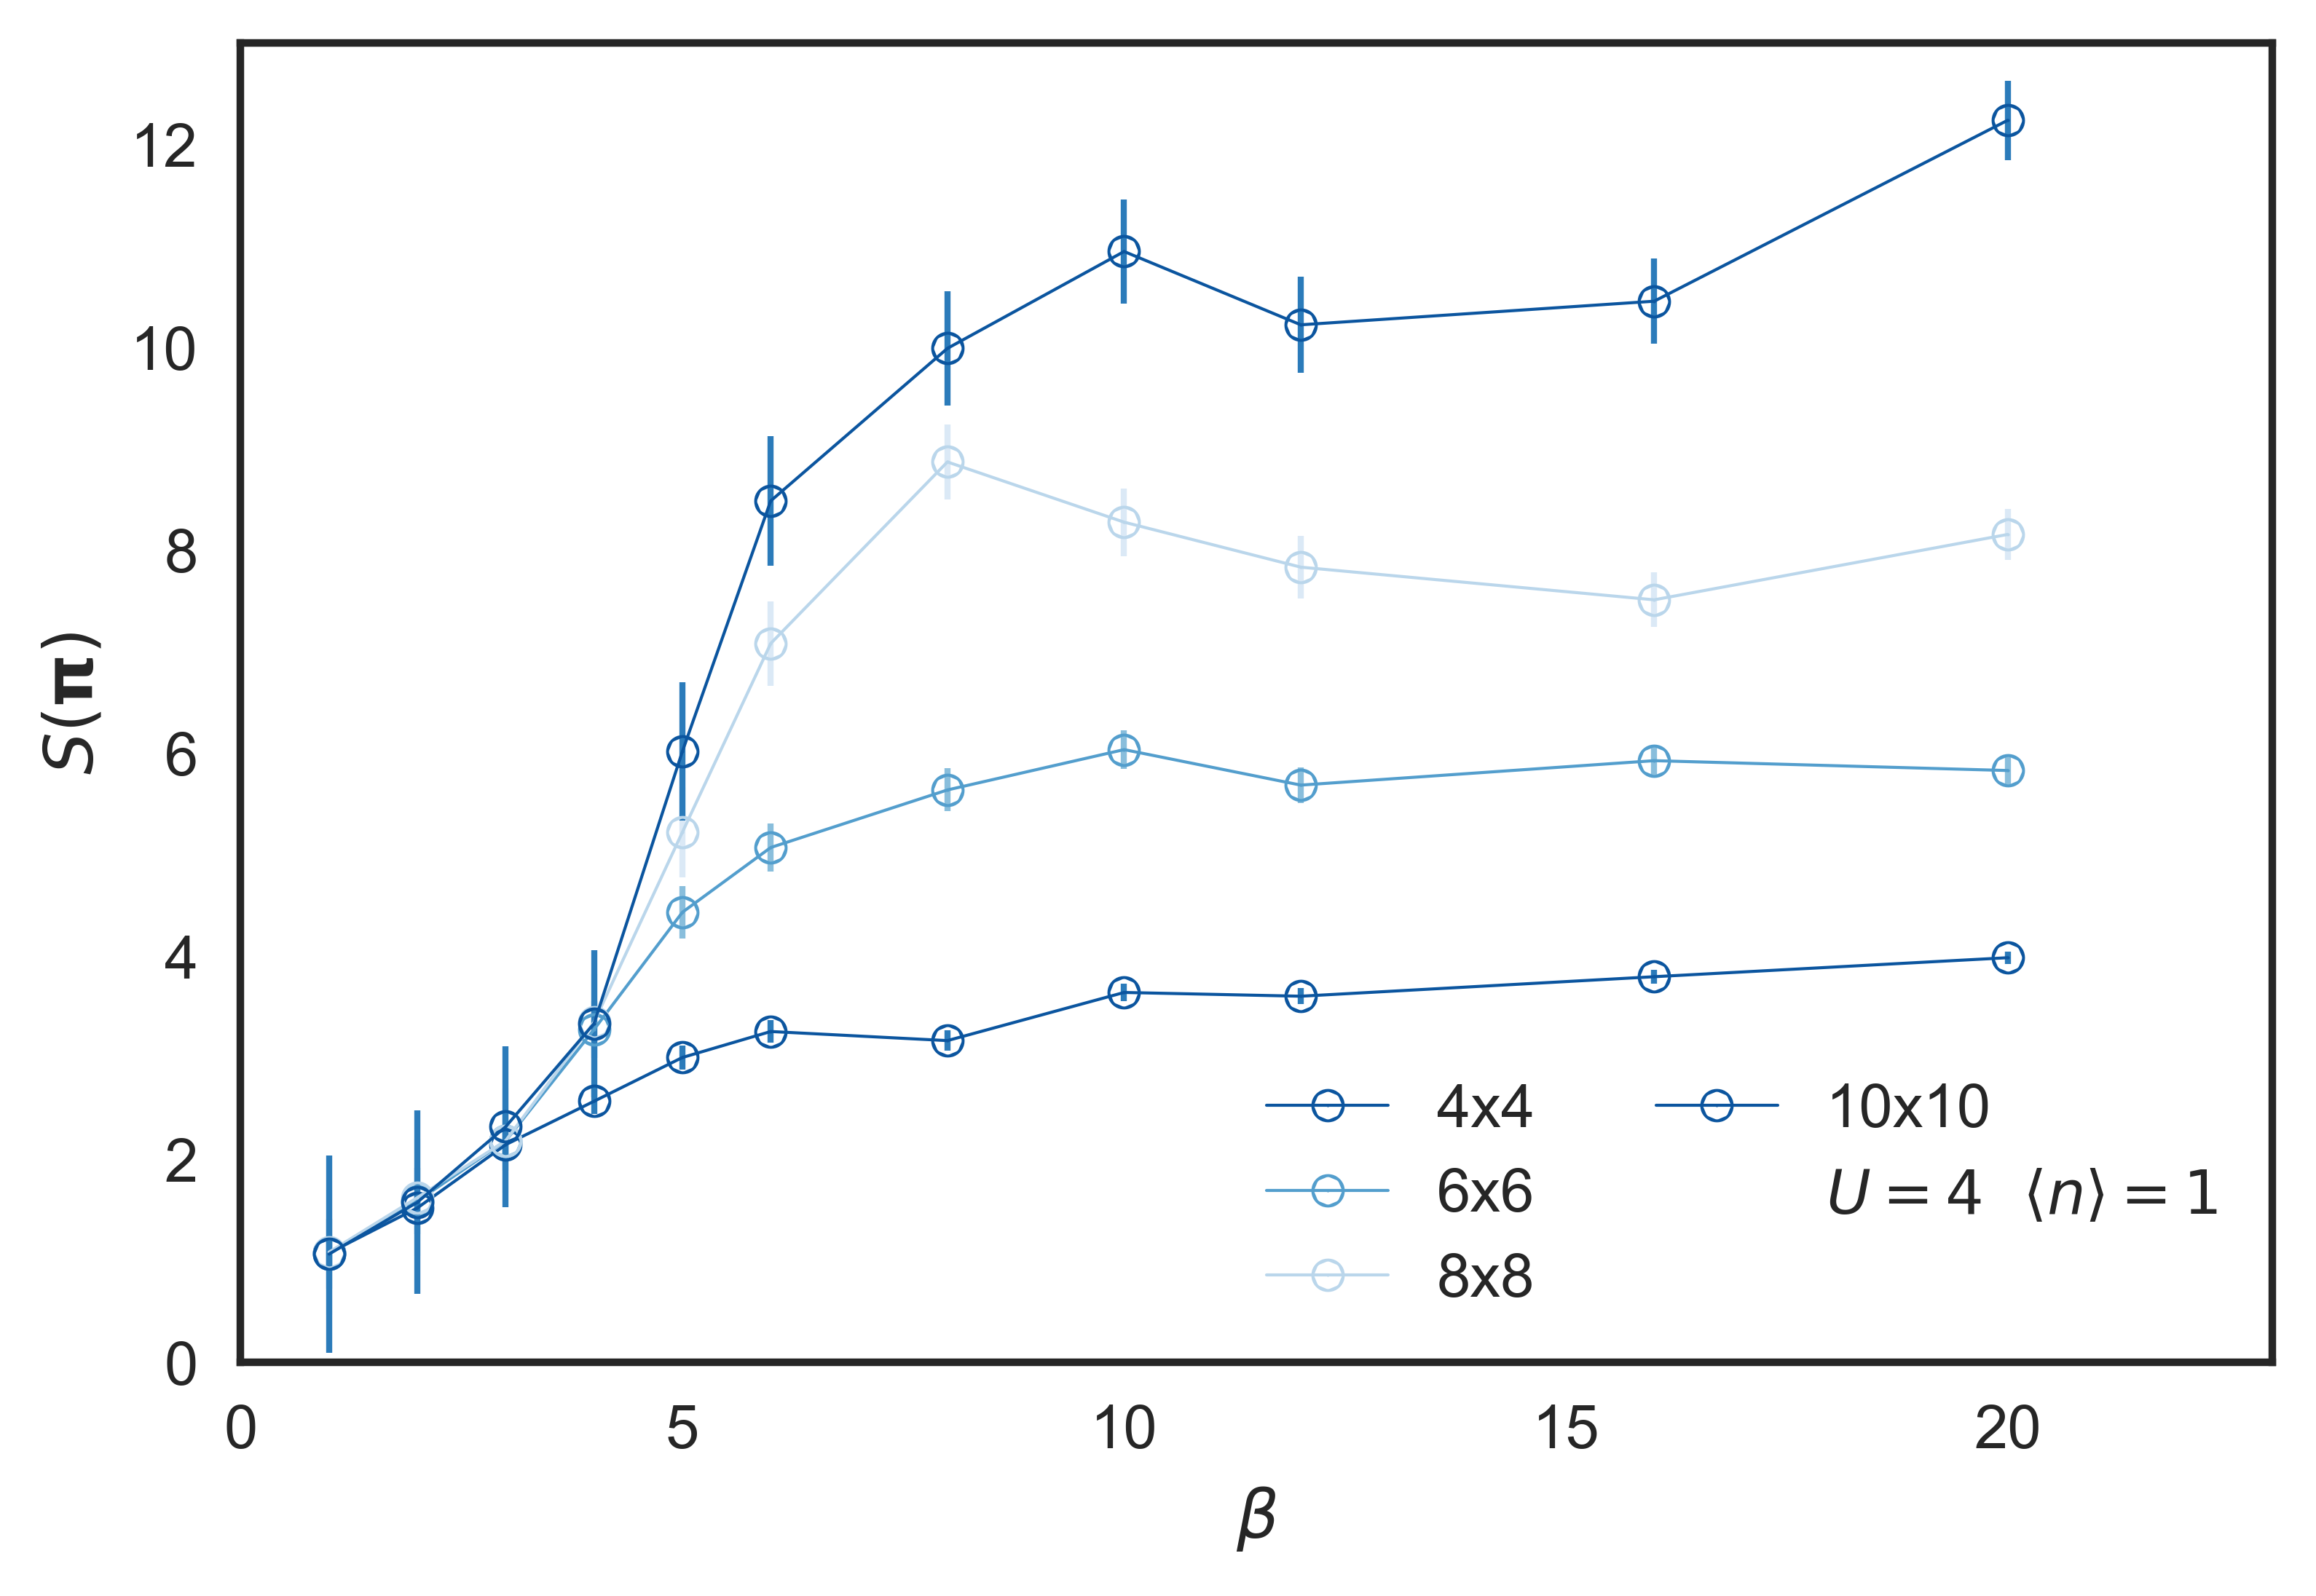
\includegraphics[scale=0.55]{Applications/square/Spipi.png}
\hspace{0.3cm}
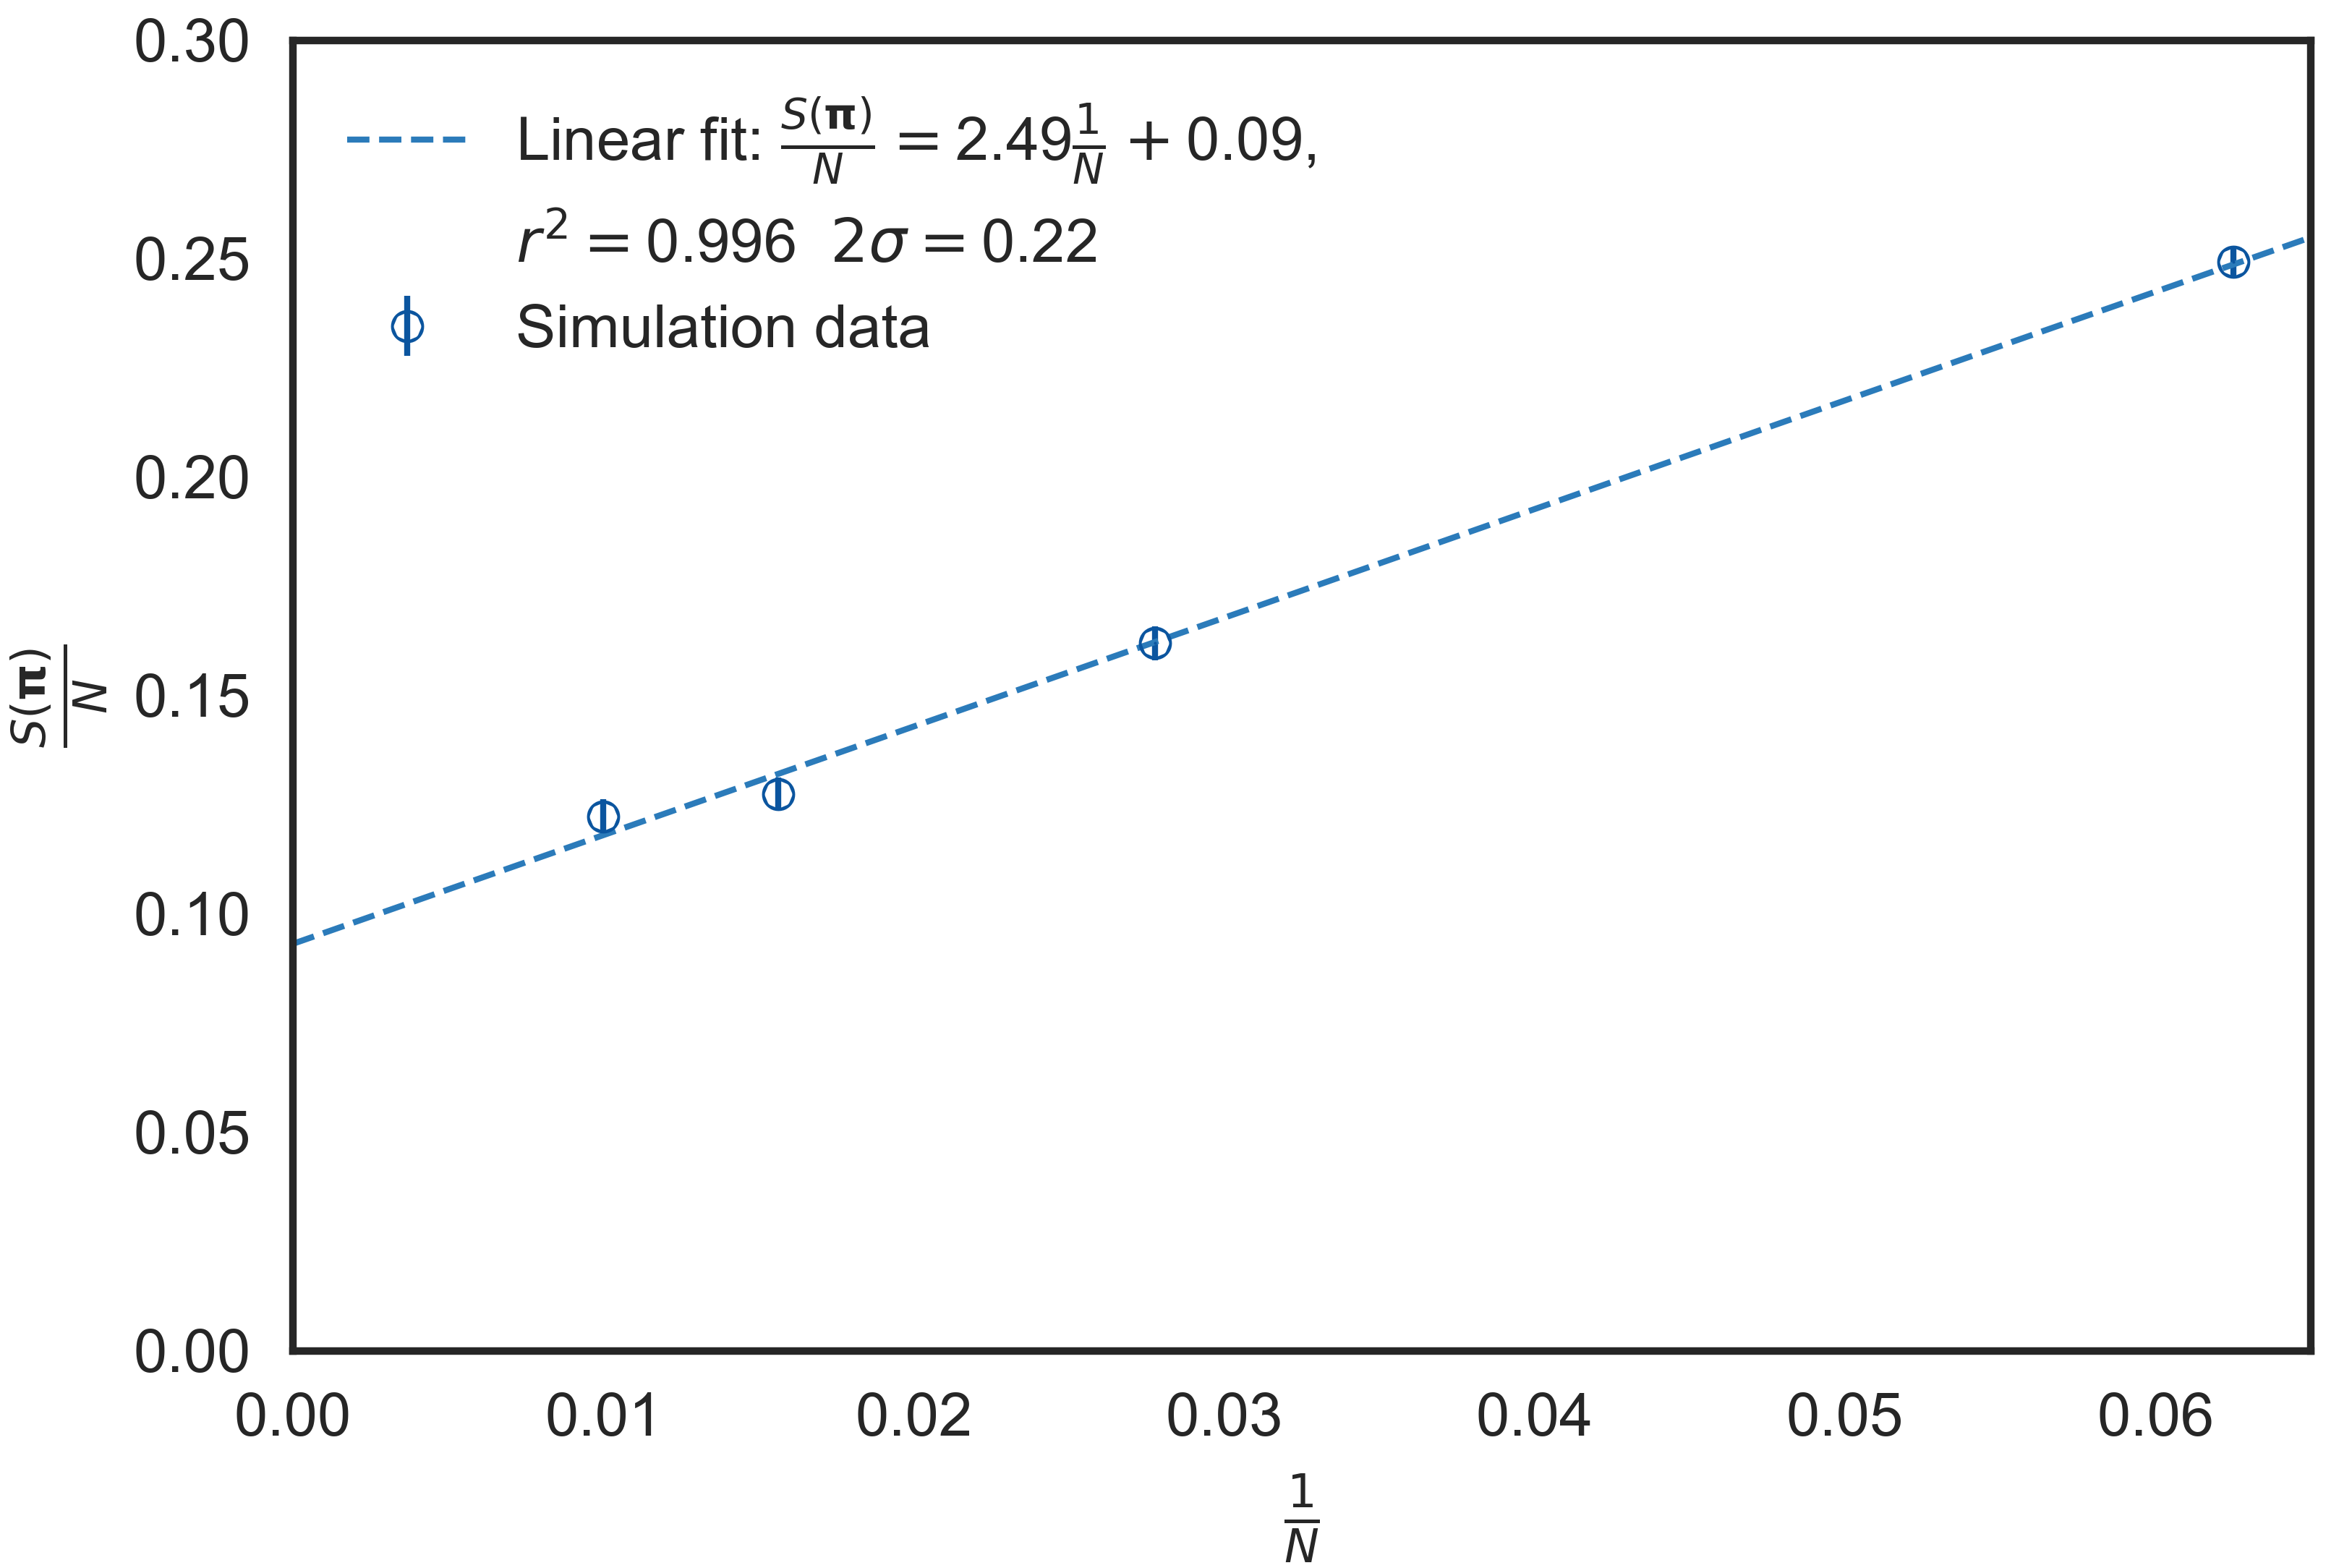
\includegraphics[scale=0.55]{Applications/square/extrapolationSpi.png}
\caption[$S ( \bm \pi ) $ for varying system size and inverse temperature.
Infinite system extrapolation of long range order.]{Left: $S ( \bm \pi ) $ for varying system size and inverse temperature.
Right: Infinite system extrapolation of long range order. \label{fig:spipi} }
\end{figure}